\chaptr{Estado del arte}{estado-del-arte}
\sect{Aplicaciones similares}{aplicaciones-similares}

Se ha realizado una búsqueda de diferentes sitios web y aplicaciones que permitan la comunicación entre usuarios a
través de un chat en tiempo real, para determinar las funcionalidades generales que ofrecen y poder tomar una decisión
sobre las nuevas funcionalidades que se implementarán en la aplicación.\ La búsqueda se ha realizado en diferentes
idiomas (español e inglés) y se han encontrado diferentes páginas web y aplicaciones que ofrecen este tipo de
servicio, que son las siguientes:

\begin{itemize}
	\item \textbf{Chateagratis.net}: Esta página web permite a los usuarios elegir un apodo (que se escoge antes de
	iniciar las conversaciones) con el que entrar en el chat, por lo que no es necesaria la creación de una cuenta de
	usuario (aunque sí que se disponga de esta funcionalidad).\ La aplicación se divide en diferentes salas, cada una
	de las cuales tiene una temática diferente y se pueden mantener múltiples salas abiertas al mismo tiempo.\ Los
	usuarios pueden unirse a las salas existentes en un listado, disponible al acceder a la aplicación o en la pestaña
	asignada para ello.\ La página web permite a los usuarios enviar solamente mensajes de texto (con ciertos
	formatos, como negrita, colores, etc.) y emoticonos, sin la posibilidad de adjuntar imágenes o archivos.\ Se pueden
	programar bots para que administren una sala y que envíen mensajes automáticos cada cierto tiempo (como el que
	se visualiza en las siguientes imágenes, designado con el prefijo @).

	\begin{figure}[H]
		\centering
		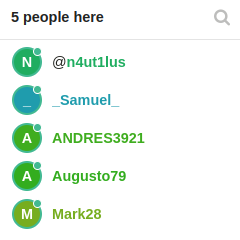
\includegraphics[scale=0.45]{ListaUsuariosChateagratis}
		\caption{Lista de usuarios conectados en una sala de chateagratis.net.}
		\label{fig:ListaUsuariosChateagratis}
	\end{figure}

	\begin{figure}[H]
		\centering
		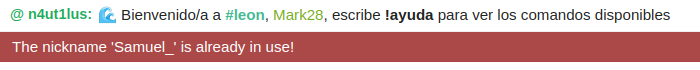
\includegraphics[scale=0.5]{ServerInfoMsgChateagratis}
		\caption{Mensajes de información del servidor en una sala de chat de chateagratis.net.}
		\label{fig:ServerInfoMsgChateagratis}
	\end{figure}

	\item \textbf{Dalechatea.me}: Esta página ofrece las mismas funciones que la anterior, pero con dos diferencias: se
	puede modificar el tamaño del chat (ancho y alto) para adaptarlo a la pantalla y necesidades del usuario y se
	pueden mandar archivos multimedia temporales (imágenes, vídeos y audios), que se borran pasados 15 minutos.
	Esta funcionalidad solo está disponible en los chats privados, no en los públicos.
	Además, se pueden agregar amigos, bloquear usuarios y añadir reacciones a mensajes de otros usuarios (como mandar
	un saludo o añadir a marcadores), entre otras funciones.

	\begin{figure}[H]
		\centering
		\raisebox{-0.4\height}{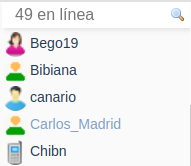
\includegraphics[scale=0.6]{ListaUsuariosDalechatea}}
		\hspace{1.5cm}
		
\includegraphics[scale=0.6]{InfoDalechatea}
		\caption{Lista de usuarios conectados y mensaje de información en una sala de chat de dalechatea.net.}
		\label{fig:UsuariosEInfoDalechatea}
	\end{figure}

	\item \textbf{Chatsfriends.com}: Esta página web ofrece las mismas funcionalidades que las anteriores, pero
	con un diseño renovado y diferente.\ Además, en la parte inferior (donde se escribe el mensaje) se muestra
	el nombre del usuario que será mostrado cuando se envíe el mensaje.\ A continuación se muestra una imagen
	de la página web, en la que se puede observar el chat en la parte central de la pantalla y un listado de
	usuarios en la parte derecha.

	\begin{figure}[H]
		\centering
		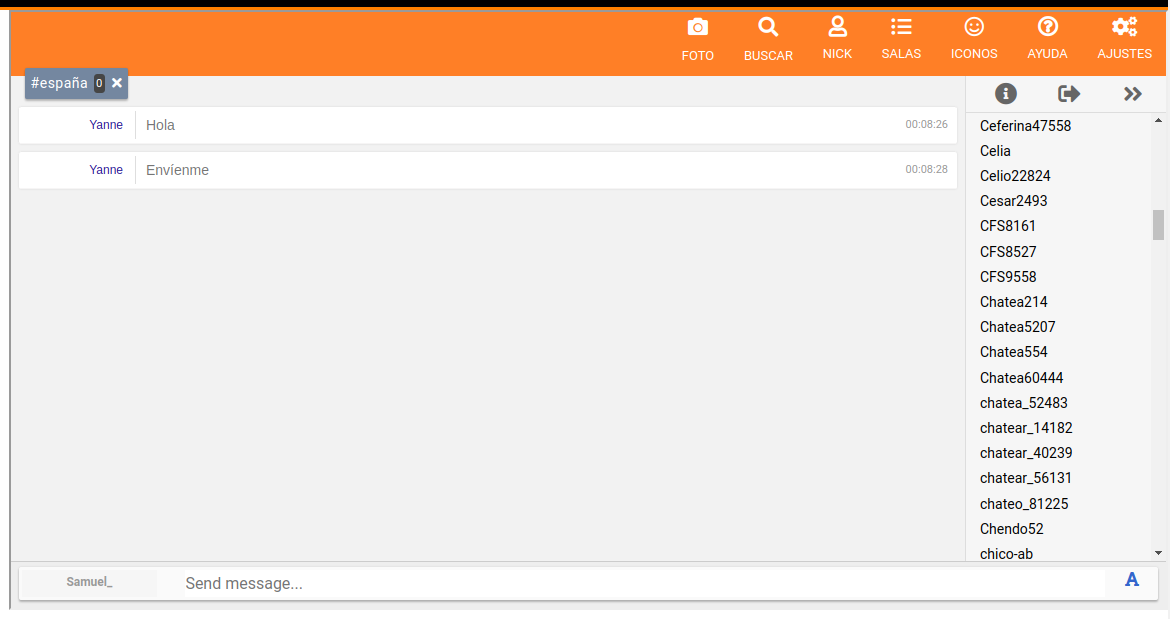
\includegraphics[width=0.8\textwidth]{Chatsfriends}
		\caption{Chat de la página web de chatsfriends.com.}
		\label{fig:Chatsfriends}
	\end{figure}
\end{itemize}
\label{itm:estadoDelArte}

Todas las páginas tienen un diseño similar, con el chat en la parte central de la pantalla y un listado de usuarios
en la parte derecha (ver imagen~\ref{fig:chatCompleto}).\ La página web de chateagratis.net tiene un diseño más
sencillo y minimalista, mientras que la de dalechatea.me tiene un diseño más moderno y con más funcionalidades.
Ambos tienen un sistema de mensajes de información, que se envían por parte del servidor del chat, para notificar a
todos los usuarios conectados al mismo de cualquier evento.\ Cuando se hace clic en un usuario de la lista, se
muestra un pequeño popup con la información del usuario seleccionado, que muestra su nombre de usuario y ciertos
botones para realizar las acciones previamente mencionadas.

% Además, en la parte inferior de la ventana de información del usuario se muestra un listado de los últimos mensajes
% enviados por el usuario seleccionado.
% Chats a los que pertenece el usuario.

\begin{figure}[H]
	\centering
	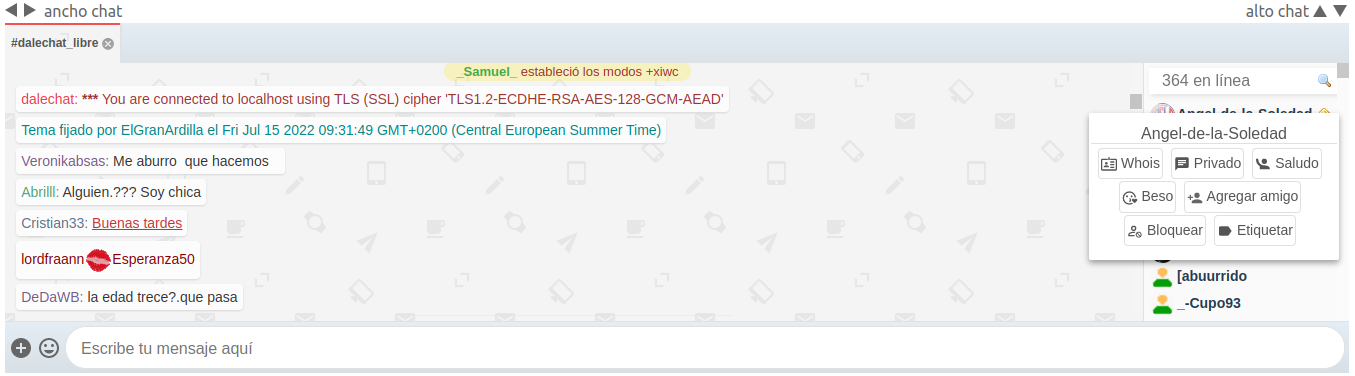
\includegraphics[scale=0.32]{Dalechatea}
	\caption{Chat completo de la página web de dalechatea.me.}
	\label{fig:chatCompleto}
\end{figure}


\sect{Opinión sobre el estado del arte}{opinion-sobre-el-estado-del-arte}

Haciendo una comparación entre las diferentes páginas web presentadas en la sección anterior, se
observa que ninguna de ellas dispone de las siguientes funcionalidades: un sistema de notificación auditiva
de mensajes recibidos, creación de grupos de chat personalizados y la posibilidad de enviar archivos
multimedia en los chats públicos.

\begin{itemize}
	\item \textbf{Notificación de mensajes}: En estas páginas web, cuando un usuario recibe un mensaje, no se le
	notifica de forma inmediata, sino que debe estar atento al chat para ver si aparece un mensaje nuevo.
	Esto puede ser molesto para los usuarios que no pueden prestar atención a la aplicación durante todo el
	tiempo que están conectados.\ Por ello, se ha decidido implementar un sistema de notificación de mensajes,
	que alerte al usuario cuando recibe un mensaje, de forma que pueda continuar con sus tareas sin tener que
	estar pendiente de la pantalla.

	\item \textbf{Creación de grupos de chat}: En la mayoría de las páginas web y aplicaciones de chat, los usuarios
	pueden unirse a salas de chat públicas, pero no pueden crear salas privadas.\ Esto puede no ser de agrado
	para algunos usuarios, que no pueden crear grupos de chat personalizados para comunicarse con sus amigos o
	familiares.\ Por ello, se ha decidido implementar un sistema de creación de grupos de chat, que permita a
	todos los usuarios crear grupos de chat personalizados para comunicarse con las personas que deseen.

	\item \textbf{Envío de archivos multimedia en los chats públicos}: En estas páginas web
	de chat, los usuarios pueden enviar distintos tipos de archivos multimedia en los chats privados, pero no en
	los públicos.\ Esto puede no satisfacer a todos los usuarios, ya que limita la comunicación entre los usuarios en
	los chats públicos.\ Por ello, se ha decidido implementar en todos los chats (ya sean públicos o privados) un
	sistema de envío de archivos multimedia.

	\item \textbf{Filtrado de imágenes inapropiadas}: En estas páginas web, los usuarios pueden enviar imágenes
	de cualquier tipo, incluyendo pornografía y otros contenidos inapropiados.\ Esto puede ser una molestia para
	la mayoría de los usuarios, que no quieren ver este tipo de imágenes.\ Por ello, se ha decidido implementar
	un sistema de filtrado de este tipo de contenido y que impida su envío en los chats.
	Además, cuando un usuario envíe un cierto número de imágenes pornográficas, se le bloqueará el acceso a la
	aplicación durante un tiempo determinado.
\end{itemize}
